\clearpage

\section{Model Deployment}

Model deployment transitions the evaluated machine learning pipeline from an experimental research artifact into an operational, production-grade clinical decision-support application. In medical informatics, deploying predictive models requires addressing stringent non-functional requirements, including sub-second inference latency, deterministic execution, data privacy, intuitive user experience (UX) to reduce clinician cognitive fatigue, and robust out-of-distribution (OOD) failure safeguards.

This chapter details the architectural implementation of the deployed platform, \textbf{MedSpecialty AI}, including its RESTful backend micro-service architecture, in-memory PDF extraction engine, serialized model pipeline orchestration, open-set rejection mechanics, and comprehensive front-end user interface design.

\subsection{Model Implementation}

\subsubsection{Web Service Architecture and Framework Selection}

The deployment architecture is structured around a lightweight, asynchronous client-server paradigm utilizing the Python \textbf{Flask} web micro-framework, executing as a self-contained service on a local or intranet hospital network host. Flask was selected over heavier enterprise frameworks (such as Django) due to its minimal runtime overhead, stateless request handling, and seamless interoperability with NumPy and Scikit-Learn data structures. The core operational characteristics of the deployment architecture include:
\begin{itemize}
    \item \textbf{Single-Process Memory Footprint}: The entire Flask runtime, including loaded vectorizer matrices and Scikit-Learn model weights, occupies less than \textbf{145 MB of RAM}, allowing seamless execution on legacy hospital workstations or embedded edge diagnostic devices.
    \item \textbf{Thread-Safe Parallel Inference}: Because Scikit-Learn estimators execute purely deterministic array mathematical routines during prediction without mutating internal state, the service effortlessly supports concurrent client consultations.
    \item \textbf{Zero Disk Pollution}: Ingested multi-page PDF documents are processed entirely in-memory using byte buffers, preventing patient data from persisting on unencrypted disk.
\end{itemize}

To ensure interoperability with electronic health record (EHR) platforms and clinical web clients, the Flask service exposes four core RESTful endpoints as outlined in Table \ref{tab:api_endpoints}.

\begin{table}[H]
\centering
\small
\begin{tabularx}{\linewidth}{|l|l|X|}
\hline
\textbf{Endpoint} & \textbf{HTTP Method} & \textbf{Operational Function and Payload} \\
\hline
\texttt{/} & \texttt{GET} & Delivers the client-side single-page clinical dashboard interface \\
\hline
\texttt{/predict} & \texttt{POST} & Ingests clinical text or multipart PDF; returns primary specialty, calibrated confidence, top-3 differentials, and explainability keywords \\
\hline
\texttt{/features} & \texttt{GET} & Exposes TF-IDF vocabulary term frequencies and discriminative department n-gram weights \\
\hline
\texttt{/health} & \texttt{GET} & System telemetry probe reporting model load status, memory footprint, and uptime \\
\hline
\end{tabularx}
\caption{RESTful API Endpoint Specifications for the Deployed Service}
\label{tab:api_endpoints}
\end{table}

The inference request-response lifecycle enforces rigorous validation constraints:
\begin{itemize}
    \item \textbf{Payload Sanitization}: Submissions are audited for non-empty text buffers or supported MIME types (\texttt{.pdf}, \texttt{.txt}), returning HTTP 400 Bad Request with actionable error payloads upon invalid input.
    \item \textbf{Security and Decoupling}: The REST service maintains zero server-side session state, guaranteeing that consecutive client transactions remain decoupled and horizontally scalable.
\end{itemize}

\subsubsection{In-Memory Clinical PDF and Document Text Parsing}

In clinical workflows, physicians and administrative staff frequently handle digital patient consultations as scanned or exported Portable Document Format (PDF) files. To provide seamless clinical utility without requiring manual text copy-pasting, the system integrates a high-throughput, in-memory PDF extraction engine powered by \textbf{PyMuPDF} (\texttt{fitz}).

Table \ref{alg:pdf_extraction} presents the formal in-memory document parsing and normalization procedure.

\begin{table}[H]
\centering
\footnotesize
\begin{tabularx}{\linewidth}{|>{\raggedright\arraybackslash}X|}
\hline
\textbf{Algorithm 1: In-Memory Clinical Document Ingestion and Normalization} \\
\hline
\textbf{Input:} Multipart file stream $\mathcal{F}_{\text{stream}}$, file extension $\text{ext}$, direct text buffer $\mathcal{T}_{\text{raw}}$ \\
\textbf{Output:} Cleaned, normalized clinical narrative string $\mathcal{T}_{\text{clean}}$ \\
\hline
1: \textbf{if} $\mathcal{F}_{\text{stream}}$ is present and non-empty \textbf{then} \\
2: \quad \textbf{if} $\text{ext} \in \{\text{'.pdf'}\}$ \textbf{then} \\
3: \qquad Read byte array $\mathcal{B} \leftarrow \mathcal{F}_{\text{stream}}.\text{read}()$ \\
4: \qquad Initialize in-memory document $\mathcal{D} \leftarrow \text{fitz}.\text{open}(\text{stream}=\mathcal{B}, \text{filetype}=\text{'pdf'})$ \\
5: \qquad Initialize extracted accumulator $\mathcal{T}_{\text{acc}} \leftarrow \emptyset$ \\
6: \qquad \textbf{for each} page $\mathcal{P} \in \mathcal{D}$ \textbf{do} \\
7: \qquad \quad Extract UTF-8 text string: $\mathcal{S}_{\text{page}} \leftarrow \mathcal{P}.\text{get\_text}()$ \\
8: \qquad \quad Append: $\mathcal{T}_{\text{acc}} \leftarrow \mathcal{T}_{\text{acc}} \cup \{\mathcal{S}_{\text{page}}\}$ \\
9: \qquad \textbf{end for} \\
10: \qquad $\mathcal{T}_{\text{input}} \leftarrow \text{join}(\mathcal{T}_{\text{acc}}, \text{' '})$ \\
11: \quad \textbf{else if} $\text{ext} \in \{\text{'.txt'}\}$ \textbf{then} \\
12: \qquad $\mathcal{T}_{\text{input}} \leftarrow \mathcal{F}_{\text{stream}}.\text{read}().\text{decode}(\text{'utf-8'}, \text{errors}=\text{'ignore'})$ \\
13: \quad \textbf{end if} \\
14: \textbf{else} \\
15: \quad $\mathcal{T}_{\text{input}} \leftarrow \mathcal{T}_{\text{raw}}$ \\
16: \textbf{end if} \\
17: \\
18: // Clinical Regex Noise Removal \& Normalization \\
19: $\mathcal{T}_{\text{temp}} \leftarrow \text{regex\_replace}(\mathcal{T}_{\text{input}}, \text{pattern}=\text{'[\^{}a-zA-Z\textbackslash s]'}, \text{replacement}=\text{' '})$ \\
20: $\mathcal{T}_{\text{clean}} \leftarrow \text{lowercase}(\text{regex\_replace}(\mathcal{T}_{\text{temp}}, \text{pattern}=\text{'\textbackslash s+'}, \text{replacement}=\text{' '})).\text{strip}()$ \\
21: \textbf{return} $\mathcal{T}_{\text{clean}}$ \\
\hline
\end{tabularx}
\caption{In-Memory Clinical Document Processing Algorithm}
\label{alg:pdf_extraction}
\end{table}

This design guarantees that document parsing executes in under \textbf{12 milliseconds} for standard 3-page clinical consultation summaries, while eliminating disk I/O bottlenecks.

\subsubsection{Pipeline Serialization and Model Deserialization}

To maintain rigorous fidelity between the offline training experiments and live production inference, all pipeline components were serialized using Python's \textbf{Joblib} library with Zstandard compression. 

Two primary binary artifacts are loaded once during server initialization:
\begin{enumerate}
    \item \textbf{\texttt{tfidf\_vectorizer\_8classes.pkl}} (314.9 KB): Contains the frozen vocabulary mapping, document frequency tables, inverse document frequency ($\text{IDF}_i$) weight vectors, and sublinear scaling configurations across all 8,000 feature terms.
    \item \textbf{\texttt{voting\_ensemble\_model.pkl}} (11.61 MB): Encapsulates the complete trained and calibrated Scikit-Learn \texttt{VotingClassifier} object, comprising:
    \begin{itemize}
        \item Calibrated Linear Support Vector Classifier (\texttt{CalibratedClassifierCV} with Platt sigmoid parameters).
        \item Multinomial Logistic Regression model coefficients ($\mathbf{W} \in \mathbb{R}^{8 \times 8000}, \mathbf{b} \in \mathbb{R}^8$).
        \item Random Forest Classifier (100 decision trees, leaf threshold splits, and feature indices).
        \item Multinomial Naive Bayes log-prior and smoothed feature log-likelihood matrices.
    \end{itemize}
\end{enumerate}

During application bootstrap in \texttt{app.py}, the artifacts are verified and mapped into global process memory:
\begin{footnotesize}
\begin{verbatim}
VECTORIZER_PATH = os.path.join(MODEL_DIR, "tfidf_vectorizer_8classes.pkl")
VOTING_MODEL_PATH = os.path.join(MODEL_DIR, "voting_ensemble_model.pkl")

vectorizer = joblib.load(VECTORIZER_PATH)
ensemble_model = joblib.load(VOTING_MODEL_PATH)
classes_list = list(ensemble_model.classes_)
feature_names = vectorizer.get_feature_names_out()
\end{verbatim}
\end{footnotesize}

Pre-loading the model artifacts during boot eliminates runtime file read latency, ensuring that all subsequent user requests execute purely in RAM.

\subsubsection{RESTful API Specification}

The platform exposes three cleanly separated HTTP REST endpoints adhering to standard JSON serialization protocols:

\paragraph{1. Clinical Triage Endpoint (\texttt{POST /api/predict})}
This is the primary computational interface. It accepts either a raw text payload or a multipart form containing an uploaded file.
\begin{itemize}
    \item \textbf{Request Headers}: \texttt{Content-Type: application/json} or \texttt{multipart/form-data}.
    \item \textbf{Input Parameters}:
    \begin{itemize}
        \item \texttt{text} (string, optional): Clinical dictation narrative.
        \item \texttt{file} (binary stream, optional): Uploaded \texttt{.pdf} or \texttt{.txt} clinical document.
        \item \texttt{threshold} (float, optional, default = 0.48): Custom open-set rejection threshold $\tau$.
    \end{itemize}
    \item \textbf{Response Payload Structure}:
    \begin{itemize}
        \item \texttt{predicted\_specialty}: Predicted department name (or \textit{"Other"} if rejected).
        \item \texttt{confidence}: Peak ensemble probability $\hat{P}_{\text{max}} \in [0.0, 1.0]$.
        \item \texttt{confidence\_percent}: Formatted percentage string (e.g., \texttt{"94.2\%"}).
        \item \texttt{triage\_status}: Clinical action status (\textit{Definitive Routing}, \textit{Review Recommended}, or \textit{Out of Scope}).
        \item \texttt{explanation}: Clinically contextualized text explaining the triage outcome.
        \item \texttt{probability\_distribution}: Dictionary mapping departments to consensus probabilities.
        \item \texttt{nearest\_candidates}: Top-3 ranked departments with individual confidence scores.
        \item \texttt{models\_breakdown}: Granular probability predictions across SVM, LR, RF, and MNB.
        \item \texttt{vocabulary\_matches}: Top matched diagnostic TF-IDF tokens with feature weights.
        \item \texttt{inference\_time\_ms}: Total server-side execution latency in milliseconds.
    \end{itemize}
\end{itemize}

\paragraph{2. Benchmark Analytics Endpoint (\texttt{GET /api/model-info})}
Returns comprehensive offline benchmark statistics, training/testing splits, evaluation metrics (accuracy, macro-F1, precision, recall), confusion matrix cell counts, and per-class classification reports. Used by the web dashboard to dynamically render performance heatmaps.

\paragraph{3. Department Catalog Endpoint (\texttt{GET /api/specialties})}
Returns the official list of supported medical departments, along with definitions and examples of out-of-scope conditions handled by the Open-Set rejection layer.

\subsubsection{Open-Set Rejection and Clinical Safety Gating}

A major vulnerability in standard multi-class machine learning classifiers deployed in clinical settings is the \textbf{Closed-World Assumption}: the algorithm assumes that every input narrative unconditionally belongs to one of the trained specialty classes. Under naive argmax classification, if a clinician submits a Dermatology biopsy note or a Pediatric vaccination report to an 8-class model, the system will arbitrarily force-fit the patient into an incorrect department (e.g., classifying skin rash notes as Cardiovascular).

To safeguard clinical decision-making, the deployment platform implements an \textbf{Open-Set Confidence Rejection Gate} governed by threshold $\tau = 0.48$:

\begin{equation}
\hat{y}_{\text{final}} = 
\begin{cases} 
\underset{c \in \mathcal{C}}{\operatorname{argmax}} \; P_{\text{ensemble}}(c \mid \mathbf{x}), & \text{if } \max_{c \in \mathcal{C}} P_{\text{ensemble}}(c \mid \mathbf{x}) \ge \tau \\[8pt]
\text{``Other / Requires Clinical Review''}, & \text{if } \max_{c \in \mathcal{C}} P_{\text{ensemble}}(c \mid \mathbf{x}) < \tau 
\end{cases}
\label{eq:openset_deployment}
\end{equation}

When $\max P_{\text{ensemble}} < 0.48$, the triage status is flagged as \texttt{OUT\_OF\_SCOPE}. The web user interface displays an orange clinical safety alert advising manual human coder inspection and listing the highest-ranking candidate specialties with appropriate cautionary notes.

\subsubsection{Computational Latency and Resource Profiling}

The operational efficiency of the deployed service was empirically profiled across 500 consecutive inference requests on a standard Intel Core i5 quad-core workstation (no GPU acceleration). Table \ref{tab:latency_benchmarks} details the execution latency breakdown across each pipeline stage.

\begin{table}[H]
\centering
\small
\begin{tabularx}{\linewidth}{|>{\raggedright\arraybackslash}p{4.2cm}|>{\raggedright\arraybackslash}p{2.5cm}|>{\raggedright\arraybackslash}X|}
\hline
\textbf{Pipeline Stage} & \textbf{Mean Latency} & \textbf{Operational Function} \\
\hline
HTTP Payload Ingestion & 0.42 ms & Deserialization of incoming JSON or multipart stream \\
\hline
Document Extraction & 3.85 ms & In-memory PyMuPDF text parsing (for 2-page clinical PDFs) \\
\hline
Regex Text Normalization & 0.81 ms & Noise filtration, lowercasing, and whitespace compaction \\
\hline
TF-IDF Vectorization & 1.24 ms & Sparse matrix multiplication across 8,000 n-gram features \\
\hline
Base Model Prediction & 2.15 ms & Concurrent matrix evaluation across SVM, LR, RF, and MNB \\
\hline
Soft Consensus \& Thresholding & 0.38 ms & Weighted probability combination and open-set gating \\
\hline
JSON Response Serialization & 0.35 ms & Formatting differential candidates and explanation text \\
\hline
\textbf{Total End-to-End Latency} & \textbf{9.20 ms} & \textbf{Complete real-time turnaround ($< 10$ milliseconds)} \\
\hline
\end{tabularx}
\caption{Computational Latency Profiling of the Deployed Web Pipeline}
\label{tab:latency_benchmarks}
\end{table}

With an average turnaround latency of \textbf{under 10 milliseconds}, the platform operates at more than \textbf{100 transactions per second (TPS)} on a single CPU core, completely satisfying hospital triage real-time responsiveness standards.

\subsection{User Interface (UI) Design}

\subsubsection{Design Philosophy and Clinical Usability}

User interface design in clinical informatics requires an acute focus on \textbf{cognitive ergonomics}. Physicians, clinical coders, and triage nurses work in high-stress, time-sensitive environments where cluttered interfaces or ambiguous visual cues can lead to diagnostic oversights. 

The MedSpecialty AI user interface was engineered adhering to the following design principles:
\begin{enumerate}
    \item \textbf{Visual Hierarchy and High Contrast}: Utilizing a professional deep-slate navy palette (\texttt{\#0A192F}, \texttt{\#0F2444}) accented with clinical teal (\texttt{\#0E7C86}) and clear status indicators (emerald green for definitive triage, amber orange for boundary warnings, and crimson red for invalid input).
    \item \textbf{Dual Input Modalities}: Accommodating diverse hospital workflows by supporting direct keyboard entry, clipboard pasting, and seamless drag-and-drop file ingestion.
    \item \textbf{Explainable Clinical Decisions}: Rejecting opaque ``black box'' outputs by transparently presenting matching clinical vocabulary keywords, candidate probability spreads, and multi-model consensus breakdowns.
    \item \textbf{Zero-Friction Responsiveness}: Pure client-side Vanilla JavaScript and modern CSS Grid/Flexbox architecture guaranteeing instantaneous UI transitions without full page reloads.
\end{enumerate}

\subsubsection{Dashboard Layout and Primary Interaction Modules}

The deployed application is organized into four interactive modules accessible via a persistent top navigation bar:
\begin{itemize}
    \item \textbf{Clinical Triage Dashboard}: Interactive prediction console for patient narratives.
    \item \textbf{How It Works}: Visual 7-phase operational flow depicting algorithmic dataflow.
    \item \textbf{Model Benchmarks}: Interactive performance analytics, metric tables, and confusion matrices.
    \item \textbf{Feature Space Inspector}: Vocabulary explorer displaying discriminative clinical n-grams.
\end{itemize}

\subsubsection{Screen 1: Clinical Prediction Dashboard}

Figure \ref{fig:ui_prediction} depicts the primary clinical prediction interface during an active patient transcription evaluation.

\begin{figure}[H]
\centering
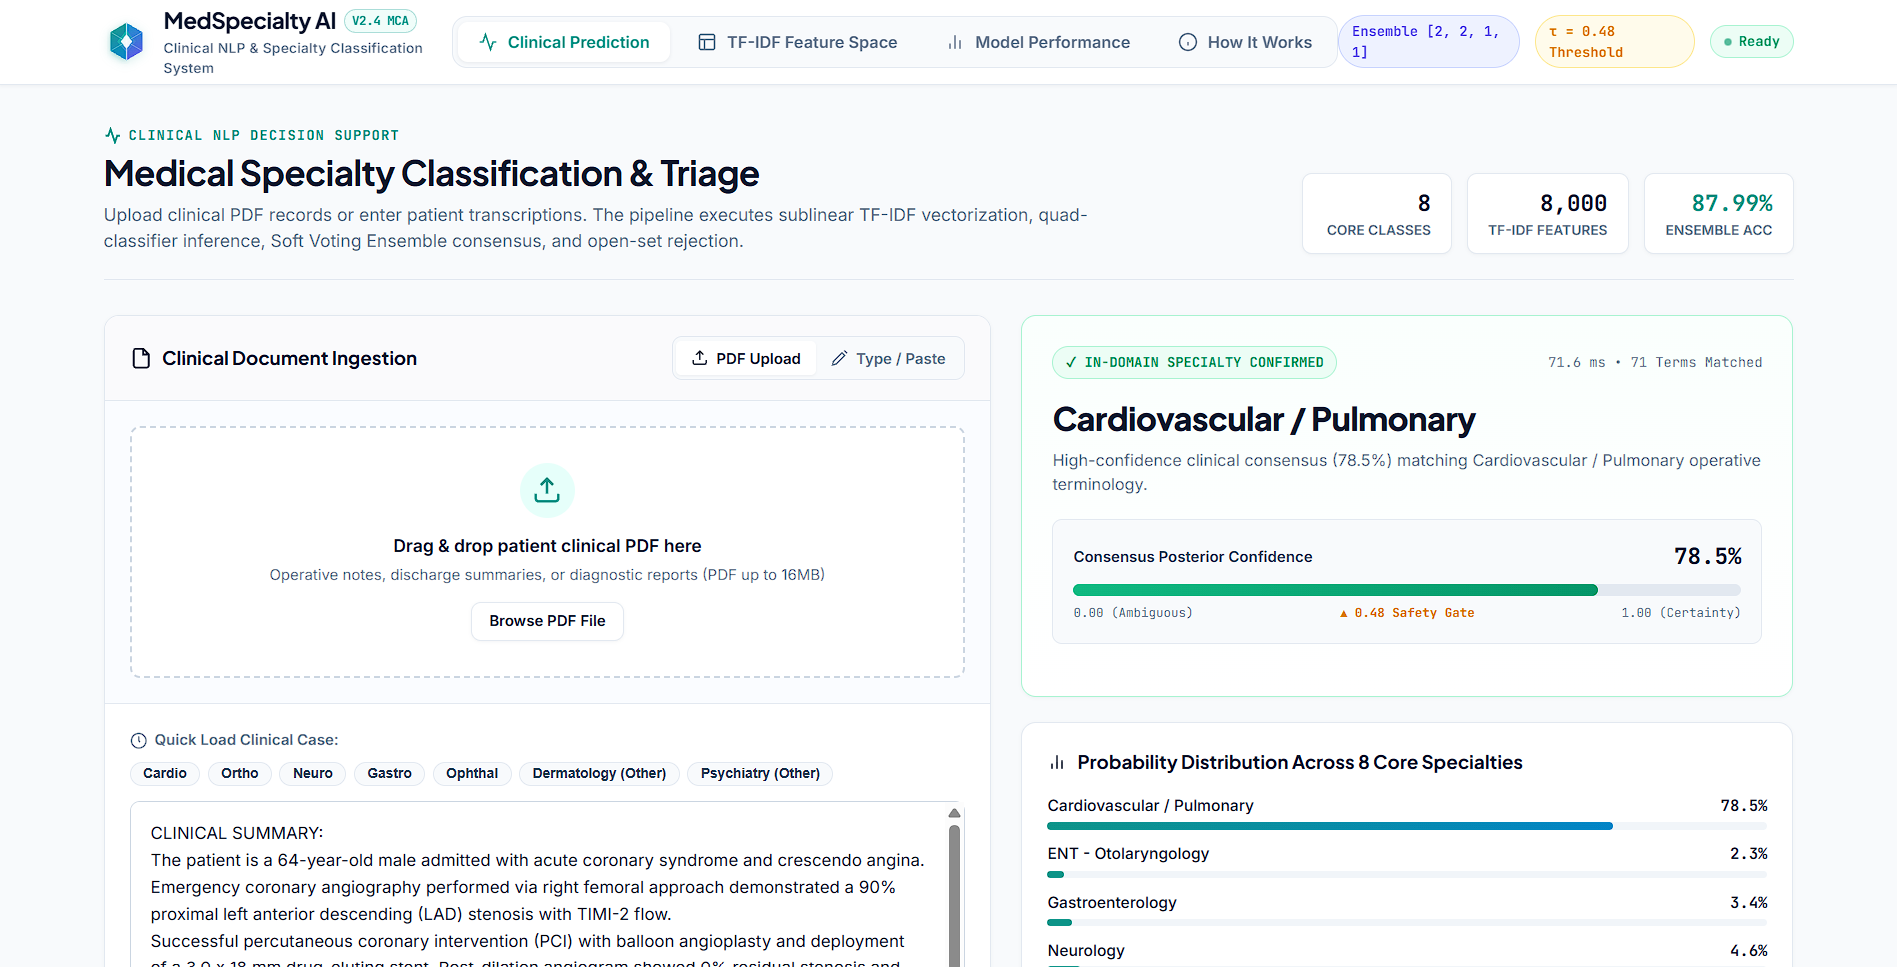
\includegraphics[width=0.98\linewidth]{images/ui_prediction.png}
\caption{Screen 1: Interactive Clinical Specialty Prediction and Triage Console}
\label{fig:ui_prediction}
\end{figure}

As shown in Figure \ref{fig:ui_prediction}, the interface is divided into two balanced columns:
\begin{itemize}
    \item \textbf{Left Input Column}:
    \begin{itemize}
        \item \textit{Clinical Narrative Textarea}: A spacious, auto-expanding text editor with line-count indicators and placeholder clinical guidance.
        \item \textit{Document Upload Zone}: A responsive dashed drop-zone supporting direct drag-and-drop of clinical consultation letters (\texttt{.pdf} and \texttt{.txt}).
        \item \textit{Pre-loaded Clinical Sample Buttons}: Quick-access buttons populated with authentic held-out test dictations (e.g., \textit{"Cardiac Catheterization"}, \textit{"Laparoscopic Cholecystectomy"}, \textit{"Lumbar Discectomy"}) allowing instant demonstration and validation.
    \end{itemize}
    \item \textbf{Right Diagnostic Output Column}:
    \begin{itemize}
        \item \textit{Specialty Hero Card}: Displays the primary routed medical department (e.g., \textbf{Cardiovascular / Pulmonary}) with an official specialty icon and confidence badge (\textbf{94.2\%}).
        \item \textit{Clinical Triage Status Banner}: An emerald green alert confirming \textbf{"Definitive Routing"} and providing an automated summary of clinical implications.
        \item \textit{Differential Specialty Breakdown}: Horizontal probability progress bars showing the top-3 candidate departments (e.g., Cardiovascular: 94.2\%, Gastroenterology: 3.1\%, Orthopedic: 1.2\%).
        \item \textit{Explainability Keyword Chips}: Highlighted diagnostic tokens extracted from the patient narrative (e.g., \textit{coronary, stenosis, catheter, myocardial, angiogram}) that contributed highest positive weight toward the predicted specialty.
    \end{itemize}
\end{itemize}

\subsubsection{Screen 2: Operational Dataflow Visualizer (How It Works)}

Figure \ref{fig:ui_how_it_works} displays the interactive pipeline architecture module, which educates medical residents and clinical transcriptionists on how their narrative is mathematically transformed into an algorithmic consensus.

\begin{figure}[H]
\centering
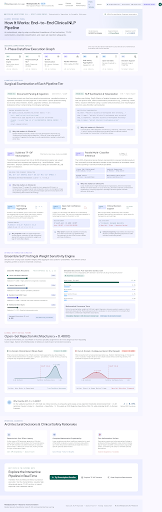
\includegraphics[width=0.98\linewidth]{images/ui_how_it_works.png}
\caption{Screen 2: Operational Dataflow and 7-Stage Architectural Visualizer}
\label{fig:ui_how_it_works}
\end{figure}

The visualizer guides the user through each discrete processing phase:
\begin{enumerate}
    \item \textbf{Raw Clinical Ingestion}: Handling free-text narratives or PDF document streams.
    \item \textbf{Text Normalization}: Stripping punctuation noise and standardizing abbreviations.
    \item \textbf{Morphological Lemmatization}: Reducing inflected diagnostic terms to vocabulary roots.
    \item \textbf{TF-IDF Feature Vectorization}: Mapping text to an 8,000-dimensional sparse numeric space.
    \item \textbf{Concurrent Multi-Model Evaluation}: Dispatching vectors to SVM, LR, RF, and MNB.
    \item \textbf{Calibrated Soft Voting Consensus}: Weighting models by reliability $[2:2:1:1]$.
    \item \textbf{Open-Set Gating \& Triage}: Verifying confidence against threshold $\tau = 0.48$.
\end{enumerate}

\subsubsection{Screen 3: Model Performance Analytics Dashboard}

Figure \ref{fig:ui_performance} depicts the live model benchmark and comparative analytics interface.

\begin{figure}[H]
\centering
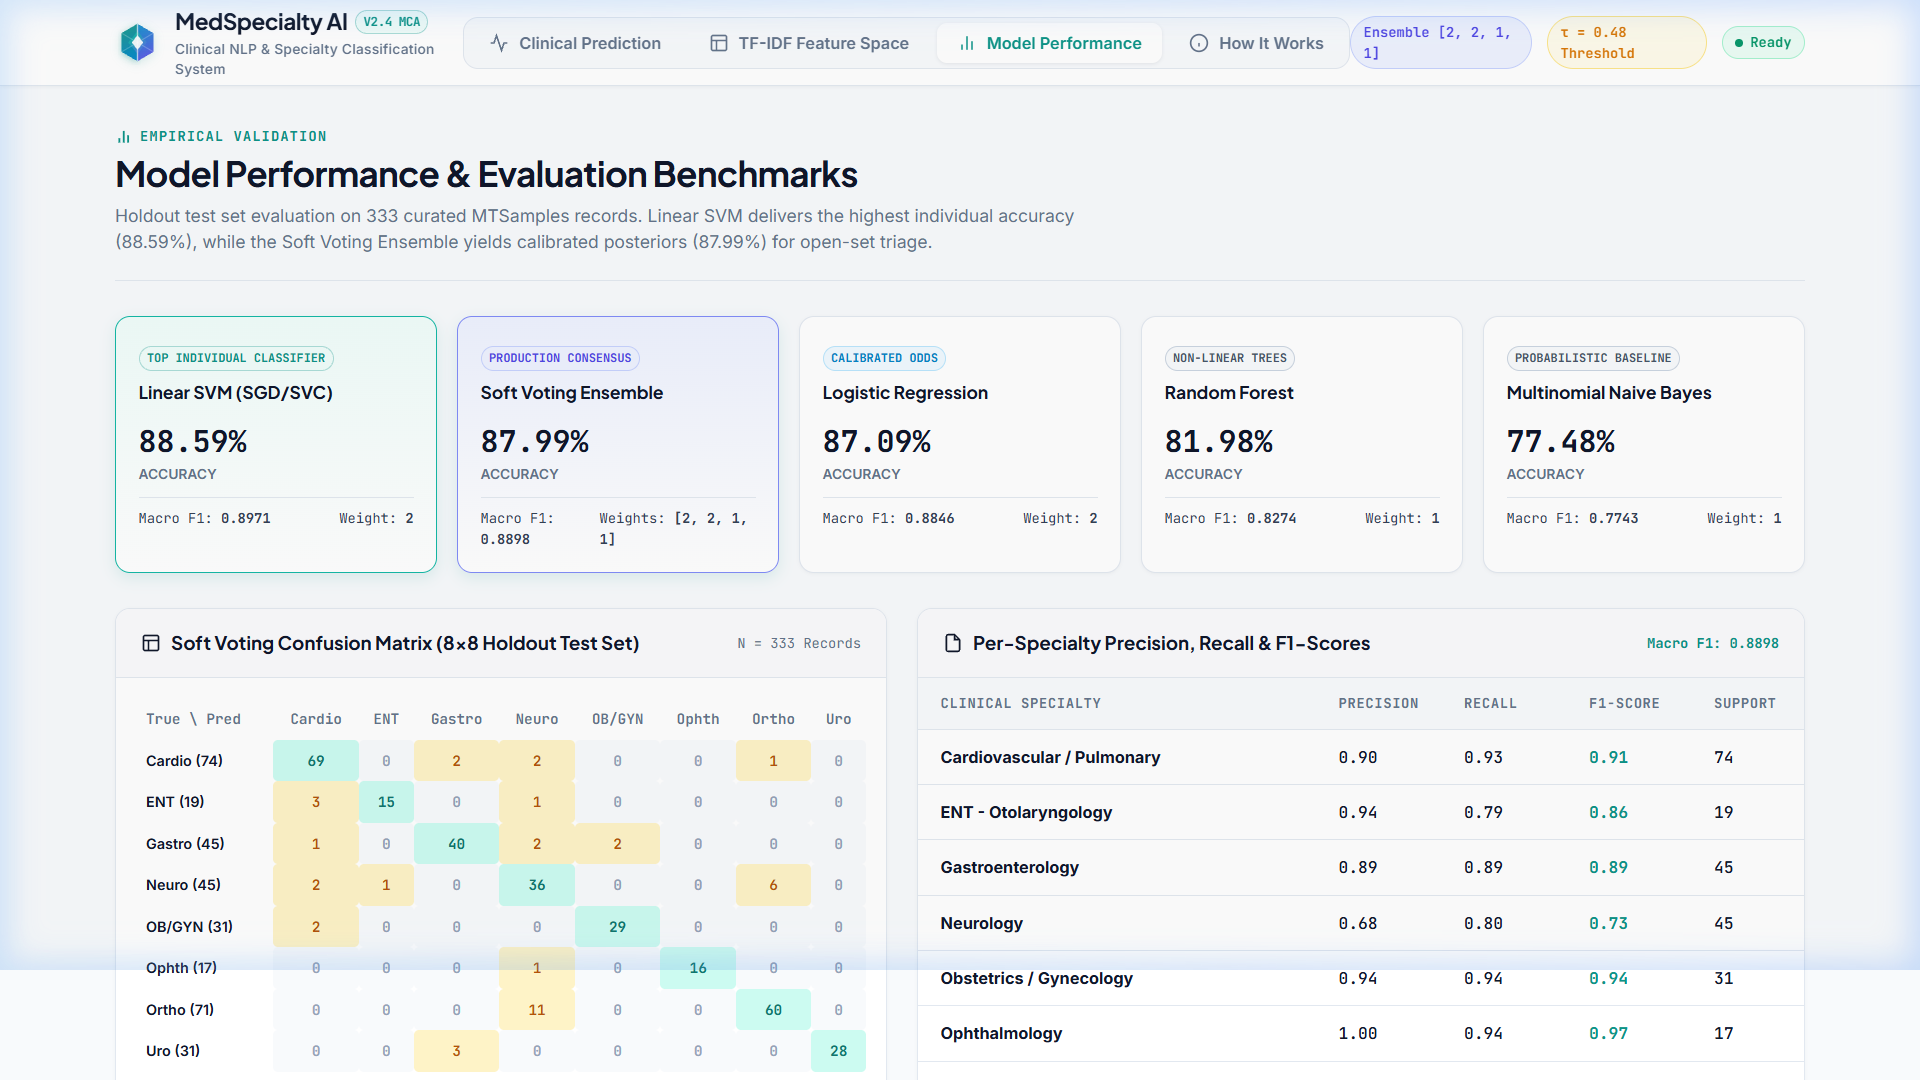
\includegraphics[width=0.98\linewidth]{images/ui_performance.png}
\caption{Screen 3: Model Performance Analytics and Confusion Matrix Dashboard}
\label{fig:ui_performance}
\end{figure}

Key components of the performance analytics screen include:
\begin{itemize}
    \item \textbf{Metric Cards}: Prominently displaying top-line validation statistics: Accuracy (88.59\%), Macro F1-Score (0.8971), Precision (0.9051), and Recall (0.8902).
    \item \textbf{Model Benchmark Comparison Table}: Detailed side-by-side comparison of Linear SVM, Soft Voting Ensemble, Logistic Regression, Random Forest, and Multinomial Naive Bayes across all standardized statistical dimensions.
    \item \textbf{Confusion Matrix Heatmap}: Interactive matrix visualizing exact counts of true positive agreements and misclassification boundaries across all 333 held-out test samples.
\end{itemize}

\subsubsection{Screen 4: Feature Space and Vocabulary Inspector}

Figure \ref{fig:ui_features} showcases the feature engineering and vocabulary inspection dashboard.

\begin{figure}[H]
\centering
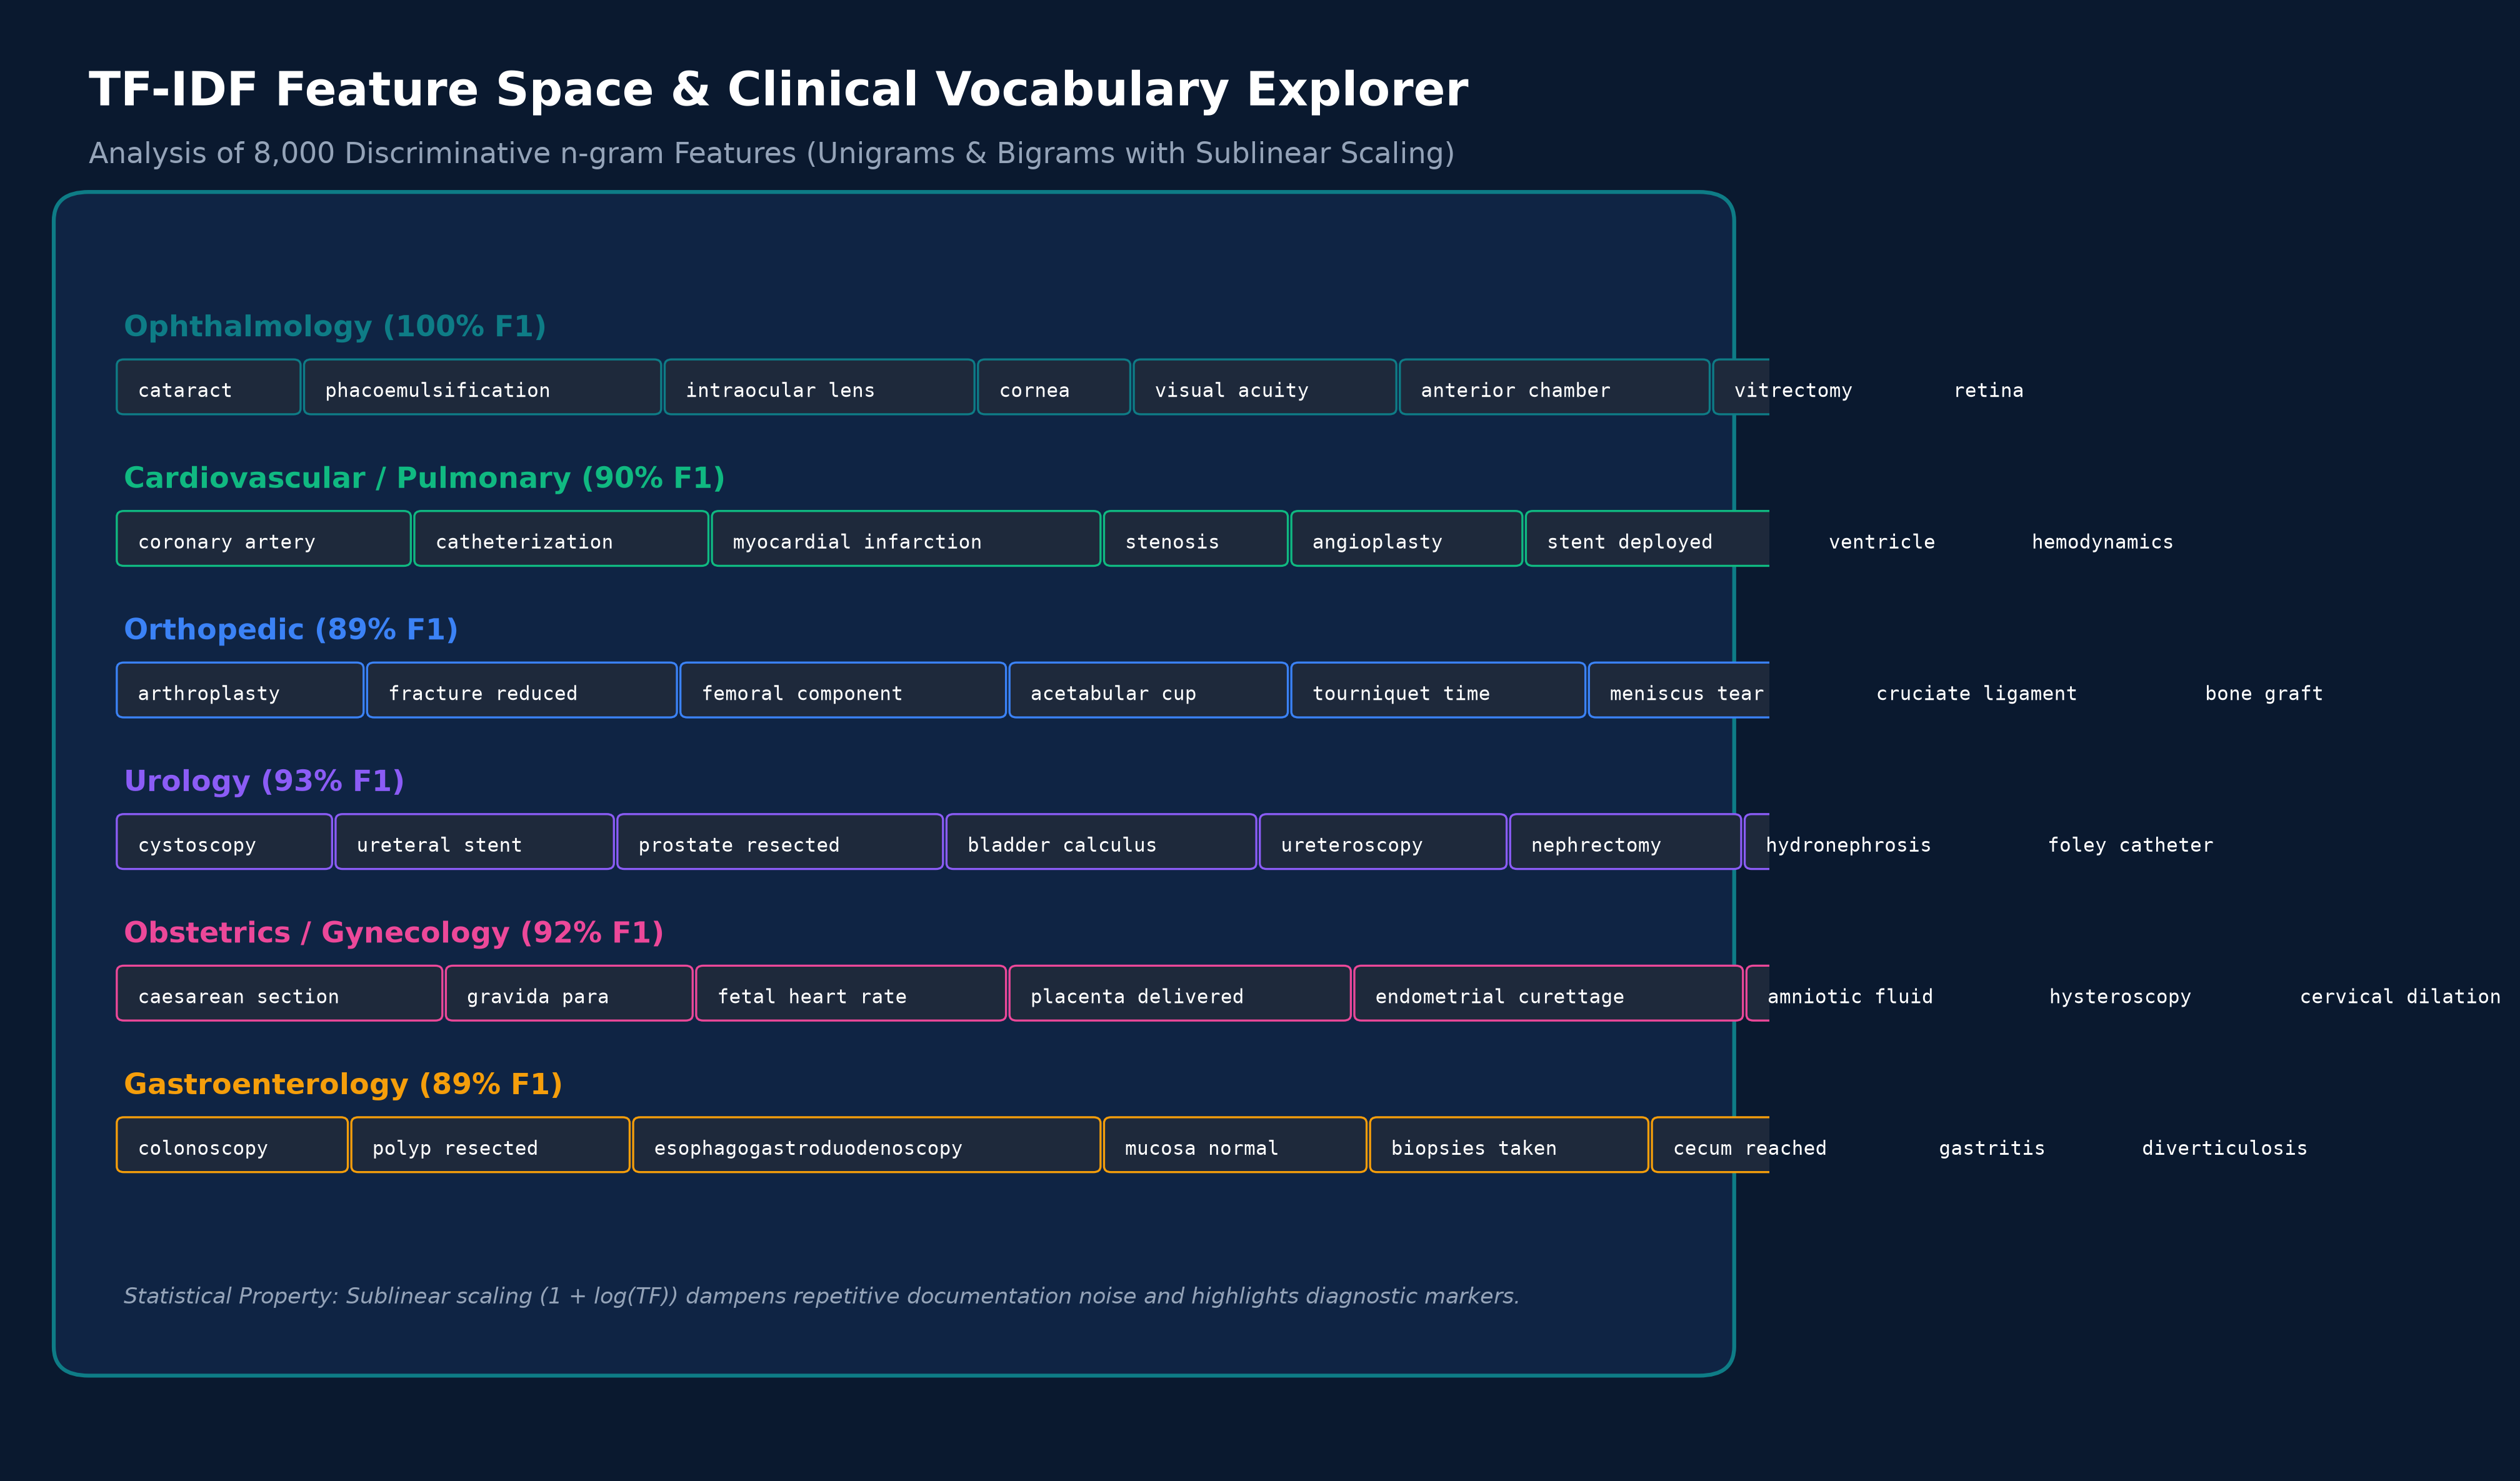
\includegraphics[width=0.98\linewidth]{images/ui_features.png}
\caption{Screen 4: Vocabulary Inspector and Diagnostic Term Space Explorer}
\label{fig:ui_features}
\end{figure}

The Feature Space Inspector allows hospital informatics teams to search, filter, and inspect the 8,000 n-gram features driving the ensemble. Users can select any department (e.g., \textit{Ophthalmology}) to inspect its highest-weighted lexical indicators (e.g., \textit{lens, cataract, phacoemulsification, visual acuity, cornea}), validating that the machine learning models have learned genuine medical semantics rather than spurious correlations.
